%% 
%% ACS project dissertation 
%% 
%% Currently designed for printing two-sided, but if you prefer to 
%% print single-sided just remove ",twoside,openright" from the 
%% \documentclass[] line below. 

\documentclass[a4paper,12pt,twoside,openright]{report}

%TODO: Title and word count
\def\authorname{Nicholas L.\ Larus-Stone\xspace}
\def\authorcollege{Queens' College\xspace}
\def\authoremail{nl363@cl.cam.ac.uk}
\def\dissertationtitle{Building a cell-free metabolic model using variational autoencoders}
\def\wordcount{10698}
\def\ecoli{\textit{E. coli}}

\usepackage{epsfig,graphicx,parskip,setspace,tabularx,xspace} 
\usepackage{gensymb}
\usepackage[acronym]{glossaries}
\usepackage[toc,page]{appendix}
\usepackage{url}
\usepackage{longtable}

\makeglossaries

\newacronym{aa}{AA}{Amino Acid}
\newacronym{ae}{AE}{Autoencoder}
\newacronym{camp}{cAMP}{Cyclic AMP}
\newacronym{cfps}{CFPS}{Cell-free Protein Synthesis}
\newacronym{coa}{CoA}{Coenzyme-A}
\newacronym{cobra}{COBRA}{Constraint-Based Reconstruction and Analysis}
\newacronym{csv}{CSV}{Comma separated Values}
\newacronym{dna}{DNA}{Deoxyribonucleic Acid}
\newacronym{ecoli}{\ecoli}{Escherichia Acid}
\newacronym{fba}{FBA}{Flux Balance Analysis}
\newacronym{gem}{GEM}{Genome scale Models}
\newacronym{hmp}{HMP}{Hexose Monophosphate}
\newacronym{k}{K}{Potassium}
\newacronym{kl}{KL}{Kullback-Leiber}
\newacronym{lb}{LB}{Lysogeny Broth}
\newacronym{lp}{LP}{Linear Programming}
\newacronym{me}{ME-Model}{Metabolic and gene Expression Models}
\newacronym{mg}{Mg}{Magnesium}
\newacronym{milp}{MILP}{Mixed Integer Linear Programming}
\newacronym{mm}{mM}{Micromolar}
\newacronym{nad}{NAD}{Nicotinamide Adenine Dinucleotide}
\newacronym{nl}{nL}{Nanoliter}
\newacronym{ntp}{NTP}{Nucleoside Triphosphate}
\newacronym{od}{OD}{Optical Density}
\newacronym{pca}{PCA}{Principal Component Analysis}
\newacronym{peg}{PEG}{Polyethylene Glycol}
\newacronym{pema}{PEMA}{Principal Element Mode Analysis}
\newacronym{relu}{ReLU}{Rectified Linear Unit}
\newacronym{rfp}{RFP}{Red Fluorescent Protein}
\newacronym{rna}{RNA}{Ribonucleic Acid}
\newacronym{tl}{TL}{Translation}
\newacronym{trna}{tRNA}{Transfer RNA}
\newacronym{tsne}{tSNE}{t-Distributed Stochastic Neighbor Embedding}
\newacronym{tx}{TX}{Transcription}
\newacronym{ul}{$\mu L$}{Microliter}
\newacronym{vae}{VAE}{Variational Autoencoder}


\begin{document}

%% FRONTMATTER (TITLE PAGE, DECLARATION, ABSTRACT, ETC) 
\pagestyle{empty}
\singlespacing
% title page information
\begin{titlepage} 

\begin{center}
\noindent
\huge
\dissertationtitle \\
\vspace*{\stretch{1}}
\end{center}

\begin{center}
\noindent
\huge
\authorname \\
\Large
\authorcollege      \\[24pt]

\includegraphics{CUni3.eps}
\end{center}

\vspace{24pt} 

\begin{center}
\noindent
\large
{\it A dissertation submitted to the University of Cambridge \\ 
in partial fulfilment of the requirements for the degree of \\ 
Master of Philosophy in Advanced Computer Science} 
\vspace*{\stretch{1}}
\end{center}

\begin{center}
\noindent
University of Cambridge \\
Department of Computer Science and Technology     \\
William Gates Building  \\
15 JJ Thomson Avenue    \\
Cambridge CB3 0FD       \\
{\sc United Kingdom}    \\
\end{center}

\begin{center}
\noindent
Email: \authoremail \\
\end{center}

\begin{center}
\noindent
\today
\end{center}

\end{titlepage} 

\newpage
\vspace*{\fill}

\onehalfspacing
\newpage
{\Huge \bf Acknowledgements}
\vspace{24pt} 

I could not have done this dissertation without the support of my two wonderful advisors Pietro Lio and Jim Haseloff.
Pietro has been consistent encouragement throughout this entire process and he never ceases to amaze me with the depth of his knowledge and perpetual enthusiam.
Jim was extraordinarily kind to let a computer scientist run around his lab for a few months and I appreciate that he let me get my hands dirty.
Both of their groups have also been extremely welcoming despite me not being in either lab full time.

Emma Talbot was my mentor in the Haseloff group and taught me everything I needed to know about the wet lab in order to get this dissertation done on time.
In Pietro's lab, Marco Barsacchi provided extremely helpful advice on how to combine VAEs and FBA and was always willing to chat.
I really appreciate both of their help.

To my Cambridge friends Tom, Harriet, Emily, and Ian: thank you for putting up with my craziness and joining me for many meals during this entire process.
Seren, thank you for the copious amounts of pesto you made me as well as your emotional support throughout this process.

Thank you also to Juanky Perdomo and my dad, James Larus, for reading drafts of this dissertation and giving me feedback.

Finally, I would like to thank all of my friends and family who encouraged me on this journey and helped me get to where I am today.
In particular, I need to thank my parents, James Larus and Diana Stone, who have nurtured my love of learning and research and put me on the track that led me here. 

\newpage
\vspace*{\fill}
\onehalfspacing
\newpage
{\Huge \bf Declaration}

\vspace{24pt} 

I \authorname of \authorcollege, being a candidate for the M.Phil in
Advanced Computer Science, hereby declare that this report and the
work described in it are my own work, unaided except as may be
specified below, and that the report does not contain material that
has already been used to any substantial extent for a comparable
purpose.

\vspace{24pt}
Total word count: \wordcount

\vspace{60pt}
\textbf{Signed}: 

\vspace{12pt}
\textbf{Date}:


\vfill

This dissertation is copyright \copyright 2018 \authorname. 
\\
All trademarks used in this dissertation are hereby acknowledged.



\newpage
\vspace*{\fill}

\singlespacing
\newpage
\dissertationtitle
{\Huge \bf Abstract}
\vspace{24pt} 

\gls{cfps} systems are a promising platform for a variety of synthetic biology applications.
These systems are simpler, faster to experiment with, and cheaper than comparable \textit{in vivo} approaches.
Despite their relative simplicity, \gls{cfps} systems lack the computational metabolic models of cell-based systems.
This dissertation provides the first end-to-end system, called \gls{sys}, that reduces a cell-based metabolic model into a \gls{cfps} model based on experimental data.
This type of model is useful for biologists who want to understand what reactions are important in their \gls{cfps} systems.

Through the creation of a system to generate these reduced models, I contribute a number of advances to the field of computational metabolic modeling and deep learning.
As one of the first applications of deep learning to metabolic modeling, \gls{sys} provides a groundwork for further exploration at the intersection of these fields.
In particular, I show that although \gls{pca} is a popular dimensionality reduction technique in computational biology, \glspl{vae} can find non-linear relationships that \gls{pca} cannot.
I also describe a \gls{vae} that we call Corr-VAE that uses a custom loss function to discover better low dimensional representations than a naive \gls{vae}.
This loss function enables our system to generate metabolic models that are sensitive to different experimental conditions.

This dissertation explores the use of \gls{sys} to create \gls{ecoli} \gls{cfps} models, but has  was designed \gls{sys} to create \gls{cfps} models for any type of \gls{cfps} system.
While Corr-VAE was designed to solve a problem relating to \gls{cfps} systems, it can be used in any biological application that generates experimental data.
Although our system was built using data from \gls{ecoli} \gls{cfps} systems, our system can be applied to \gls{cfps} systems derived from any organism that has a \gls{gem}.
This work will lead to new ways to configure and monitor cell-free systems and will be useful to wet lab biologists.

\newpage
\vspace*{\fill}


\pagenumbering{roman}
\setcounter{page}{0}
\pagestyle{plain}
\tableofcontents
\listoffigures
\listoftables
\printglossaries

%\let\cleardoublepage\cleardoublepage

\onehalfspacing

%% START OF MAIN TEXT 

\chapter{Introduction}
\pagenumbering{arabic} 
\setcounter{page}{1} 

%TODO name our system

Despite more than a century of active biology research, many biological systems lack good computational models.
Computational models are useful if they accurately capture how the underlying biological system behaves.
When these models are faithful to the underlying biology, experiments can be run \textit{in silico} instead of \textit{in vivo}, speeding up the pace of research.
%A good model should also be consistent---running it multiple times should produce the same results.
%Though biological experiments can have wide variance due to external conditions, we want our model to vary only due to intrinsic biological sources of variation.
%Exact reproducibility is very difficult in laboratory environments, but a computer model can and should eliminate the extrinsic sources of variance that one encounters in a laboratory setting.
Moreover, the best computational models are useful not only as biology simulators, but also as facilitators of new hypotheses.
Computational biology models should both help researchers improve their understanding of the modeled system and expose novel insights into the underlying biology.

%TODO: maybe remove?
%Recent efforts to model biological systems have become ever more accurate as the amount of biological data collected increases.
Biological systems are complex and can be examined at various levels of abstraction.
For example, one model could use a physical description of a cell to predict its shape as it grows.
A different model could use -omic data---genomic, transcriptomic, and metabolomic measurements---to model the production of compounds that allow for cellular growth.
Our efforts focus on modeling the metabolism of a biological system to help biologists better understand what reactions are occurring in that system.
%As all models are inherently limited in some way, so the choice of the type of model that is used to describe a system is extremely important.

Our goal is to provide a metabolic model of a \gls{cfps} system that is useful for biologists working with \gls{cfps} systems.
This dissertation details an end-to-end system that produces metabolic models for \gls{cfps} systems from experimental data.
Our system learns which reactions are most important for a given cell-free system and produces a reduced metabolic model that fits the experimental data.
We utilize a Variational Autoencoder (\gls{vae}) on top of a common metabolic modeling technique called Flux Balance Analysis (\gls{fba}) to produce these reduced models.
In particular, we introduce a new loss function based on correlation with experimental data for our \gls{vae}.
We call this new model a Corr-VAE.
The Corr-VAE perturbs the latent space of a \gls{vae} to better fit our experimental data.
Our system can be used by biologists to navigate the parameter space of different starting conditions, cope with batch variation, and gain a deeper understand of the composition of cell-free systems.

\begin{figure}[t!]
\begin{center}
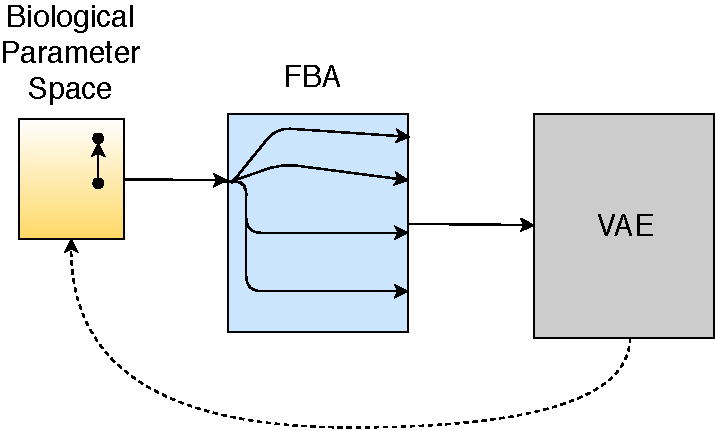
\includegraphics[width=\textwidth]{figs/FBA_Amplifier.pdf}
\end{center}
\caption[High-level idea behind our system]{High-level idea behind our system.
Small changes in the parameter space are amplified across many different fluxes in a \gls{fba} model.
We used a \gls{vae} to understand how the changes in the fluxes reflect the changes in the parameter space. 
}
\label{fig:fba_amp}
\end{figure}

\textbf{Metabolic models}

%TODO: fix this paragraph--why is it relevant/here?
Metabolism is defined as all of the chemical reactions that occur within an entity---usually an organism or a cell---in order to sustain its life and growth.
Biologists are interested in understanding how different parts of metabolism function, as metabolic reactions are the end result of the other biological process of interest (e.g. transcription and translation).
While ongoing work continues to develop a more robust understanding of metabolism, recent advances have begun to explore applications that involve manipulating the metabolism. 
Metabolic engineering has the potential to create novel advances in medicine and energy production such as increased bioproduction of the antimalarial drug artemisin~\cite{keasling2012synthetic}.
Metabolic models are an important tool for metabolic engineers because they can be used to predict how the phenotype of an organism will respond to manipulation.

%TODO: fix this sentence
Most metabolic models represent the chemical reactions in a cell with a mathematical representation of the reaction coefficients.
Individual reactions are denoted as equations in these models.
Mathematical constraints are placed on these reactions based on our knowledge of biological pathways.
Models of this type are collected under the heading of \gls{cobra} models~\cite{schellenberger2011quantitative} and are very common in the metabolic engineering community~\cite{orth2010flux}.
One of the most popular constraint-based metabolic models is \gls{fba}.
It has been used in hundreds of different works to model metabolism~\cite{feist2008growing}.
These applications range from optimizing metabolic pathways~\cite{almaas2004global} to investigating gene networks~\cite{shlomi2007genome}.
\gls{fba} is based on a genome-scale metabolic models (\glspl{gem}) reconstructed from the genome of an organism of interest.
However, these \glspl{gem} describe living organisms, not cell-free systems, so typical \gls{fba} models cannot be applied out of the box to a cell-free system.

In addition, since metabolism is a heterogenous mixture of reactions, small changes in the parameter space can lead to large changes in the metabolic output of a system.
The parameter space for \gls{cfps} systems primarily consists of final concentrations of energy substrates.
Current models are unable to explain how changes in the concentration of a certain reactant will affect the output of a \gls{cfps} system.
Even using a modeling technique such as \gls{fba} will not solve this issue because \gls{fba} acts as a non-linear amplifier on small changes in the parameter space.
We use a \gls{vae} to understand how the changes in the original parameter space are reflected in the output of a \gls{fba} model.
Figure \ref{fig:fba_amp} illustrates how our system can be used to 

Building this type of learning system requires datasets that explore across a biologically relevant parameter space.
These datasets are not common, so this dissertation required extensive experimental work in order to generate data that could be used to learn a model.
We will be also be releasing the \gls{cfps} datasets we generated to aid with further modeling work of \gls{cfps} systems.
Additionally, performing both the experimental work and the modeling allowed us to acquire a deep understanding of the data we were generating.
Without this understanding, building biologically relevant models would be difficult.

\textbf{Cell-free systems}

A Cell-free Protein Synthesis (\gls{cfps}) system is a reduced version of a cell that produces proteins without being alive.
The Central Dogma of biology, as enunciated by Francis Crick, is that \gls{dna} makes \gls{rna} makes protein~\cite{crick1970central}.
While this may be a slight oversimplification, the key idea is that the production of proteins is the end goal for most biological systems.
\gls{cfps} systems take that to an extreme by removing all endogenous \gls{dna}, \gls{rna}, and membranes while retaining the machinery for transcription and translation.

A \gls{cfps} system is therefore a type of programmable matter, a veritable biological computer.
The \gls{cfps} system acts like a computer because it can `execute` any \gls{dna} `program` that is added to the mixture.
The output of a \gls{cfps} system is determined by which \gls{dna} program is loaded into a cell-free system.
This simplicity has made cell-free systems popular for a wide array of applications~\cite{hodgman2012cell, rollin2013new, carlson2012cell}.
Additionally, cell-free systems have been shown to be extremely cheap, costing less than \$0.01 per \gls{ul} of reaction~\cite{sun2013protocols, murray2013cost}.

\gls{cfps} systems have two key aspects that make them an ideal platform to model for this dissertation.
First of all, running experiments in a \gls{cfps} system is much faster than typical \textit{in vivo} methods because performing an experiment does not require growing cells.
This meant that we were able to start from scratch and generate relevant data within several weeks instead of the many months or years for a cell-based system.
\gls{cfps} systems are also simpler than a full cellular system and should therefore be easier to model accurately.
By definition, \gls{cfps} systems are composed of blended cells and contain a strict subset of the reactions that occur in a cell-based system.
The key issue is that we do not know which reactions are included in that subset.

The unknown composition of cell-free systems means that despite their reduced complexity, \gls{cfps} systems lack good models.
However, prior attempts at modeling \gls{cfps} systems have used metabolic models to examine \gls{cfps} systems.
We believe that metabolic models are a natural fit for modeling \gls{cfps} systems.
Since \gls{cfps} are not living organisms, their effectiveness is entirely based on reaction constraints and energy regeneration.
Thus, understanding the metabolism of these systems is extremely important.
The few existing metabolic models for \gls{cfps} systems have been hand-constructed by a specific lab~\cite{bujara2012silico, vilkhovoy2017sequence}.
We provide an automated system to reduce standard \glspl{gem} to metabolic models of \gls{cfps} systems.

\textbf{Contributions}

This dissertation makes a number of contributions in the field of metabolic modeling and dimensionality reduction for \gls{cfps} systems.
\begin{itemize}
\item We provide one of the first applications of deep learning to metabolic models.
We show that using a \gls{vae} is more effective than \gls{pca} with regards to building a reduced metabolic model.
Since \gls{pca} is a common dimensionality reduction technique in biology, this motivates other work to consider using \glspl{vae} instead of \gls{pca}.
\item Corr-VAE is a new loss function for \glspl{vae} that incorporates a correlation loss term.
Although Corr-VAE was developed specifically for use with experimental data generated from \gls{cfps} systems, the structure of the network does not require it to be used only with cell-free systems.
Corr-VAE can be used in other biological application that generate experimental data and have a need for dimensionality reduction.
\item Finally, we produce a number of new, reduced models for \gls{cfps} systems.
These models more accurately describe \gls{cfps} metabolism than full-scale \glspl{gem} and can be used by biologists and metabolic engineers working with these \gls{cfps} systems.
%\item Finally, we uncovered a number of biological insights
%\item This dissertation provides an end-to-end system to generate models for \gls{cfps} systems.
%Given biological data generated in a lab, the computational pipeline will then produce a metabolic model for the given \gls{cfps} system.
%\item Within that framework, we provide a the first automated reduction system that tailors \glspl{gem} specifically for \gls{cfps} systems.
%That means our system can be used for any cell-free system that is derived from an organism that has a fully specified GEM, of which there are many dozens.
%\item Additionally, this is one of the first applications of deep learning or autoencoders to \gls{fba} models.
%As deep learning becomes ever more popular, our system provide an early example of how it may be incorporated into the field of metabolic modeling.
\end{itemize}
%VAE
%experiments + computational
%latent representation
We note that our approach was designed to be as general as possible, which has two key benefits.
Our system can be applied out-of-the-box to other types of cell-free systems; i.e. systems that use cells from organisms other than \gls{ecoli}.
Additionally, the techniques developed here for modeling cell-free systems can be applied to modeling other biological systems that uses experimental data and metabolic models.

\textbf{Outline}
\begin{figure}[t!]
\begin{center}
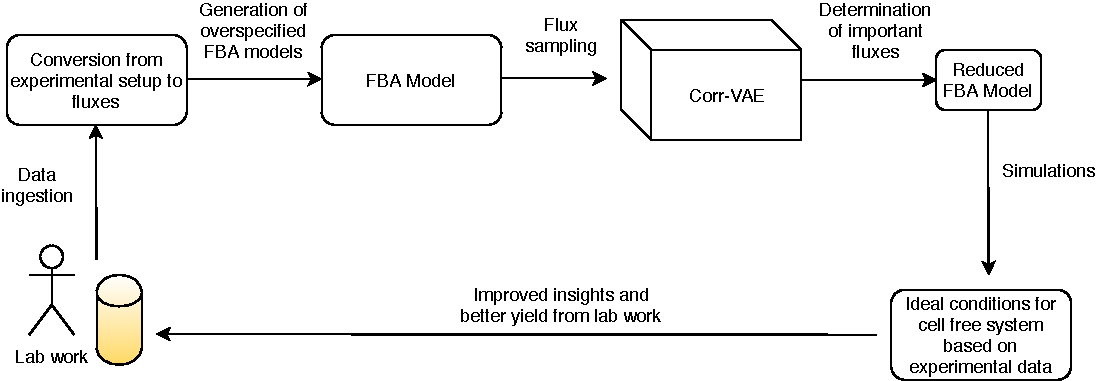
\includegraphics[width=\textwidth]{figs/SystemOverview.pdf}
\end{center}
\caption[The overall pipeline for our system]{The overall pipeline for our system.
Given experimental data on one end, we are able to generate cell-free metabolic models.}
\label{fig:overview}
\end{figure}

The structure of this dissertation is as follows.
%TODO add back in?
Chapter \ref{chap:bkg} provides background information on cell-free systems, \gls{fba}, and \glspl{vae}.
%We describe the different types of cell-free systems, how we produce our system, and some uses and advantages for cell-free systems.
%Then, we explore the mathematical foundations of \gls{fba} and how it can be used to model biological systems.
%Finally, we explain how autoencoders are used for dimensionality reduction, specifically focusing on how VAEs work.
Chapter \ref{chap:rw} provides related work in the fields of metabolic models, reduction of metabolic models, modeling cell-free systems, and \glspl{vae}.
%We analyze the current state of the art in metabolic modeling, specifically focusing on the development of \gls{fba} and the creation of a GEM for \ecoli.
%Next, we focus on how search techniques have been used to reduce metabolic models to their core reactions.
%Then, we share efforts to model cell-free systems, describing two prior works that have applied \gls{fba} to cell-free systems.
%Finally, we outline the relevant literature about VAEs.
Chapter \ref{chap:impl} describes the system we have designed and built to model cell-free systems (shown in Figure \ref{fig:overview}).
%We begin by describing our experimental setup and how we generated our data.
%Next, we detail how to ingest the experimental setup and data and convert it into a metabolic model.
%Then, we explain how we used that model to generate a larger dataset for our deep learning algorithms.
%Lastly, we use that dataset to train a VAE, which generates a lower dimensionality representation that can be used to create better cell-free metabolic models.
Chapter \ref{chap:res} describes the results of using a \gls{vae} to reduce \gls{fba} models.
Notably, we show that our reduced models are better at describing \gls{cfps} systems than both \glspl{gem} and already published reduced models.
%We also show novel biological insights that were unearthed due to my system.
%Finally, we illustrate how a model can be learned on one set of biological data and transfer to a different set of data. 
We conclude with a discussion of future work in this area.


\chapter{Background}\label{chap:bkg}

%TODO more math and explain it

\section{Cell-free systems}
\gls{cfps} systems have existed since the early 1960's as a way to express proteins that are otherwise difficult to express in a living cell~\cite{nirenberg1961dependence}.
These early \gls{cfps} systems were quite crude and had low protein yields, limiting their utility.
More recently, work involving the removal of certain genes~\cite{calhoun2006total} and the improved stability of cofactor regeneration pathways~\cite{jewett2008integrated} has allowed for improved yield of \gls{cfps} systems.
%stabilized amino acid synthesis leading to 
%Another crucial development was the ability to ensure cofactor regeneration pathways were maintained in the \gls{cfps} system}.
%These recent improvements in \gls{cfps} systems have led to a multitude of applications for cell-free technologies~\cite{}.

When discussing \gls{cfps} systems, it is important to distinguish between the multiple types of cell-free systems.
One type of cell-free system is created by combining individual purified proteins involved in transcription and translation.
The most widely utilized of these reconstituted cell-free systems is the PURE system~\cite{shimizu2001cell}.
The benefit of these systems is that the system is completely known and controlled.
Since the only things in the system are the proteins that have been deliberately aded, users of the systems can be assured that there are no undesirable elements such as nucleases or proteases present.
However, these systems have relatively high costs due to the time and effort required to isolate and purify each of the requisite proteins.

The type of \gls{cfps} system we use in this dissertation is an extract-based system created using a crude cell extract.
Creating an extract-based \gls{cfps} system involves growing cells and then lysing them to create a cell extract.
This extract is then used as the basis of the \gls{cfps} system with the assumption that all the important transcription/translation machinery remains intact in the cell extract.
Growing up large quantities of cells is relatively cheap, so these types of systems have the potential to scale more effectively than reconstituted cell-free systems. 
The downside to this method of creating \gls{cfps} systems is that the exact composition of these cell extracts is unknown and could potentially vary between batches of \gls{cfps} systems.
This motivates our work to provide an accurate model of these crude \gls{cfps} systems.

\section{Flux Balance Analysis}
Flux Balance Analysis (\gls{fba}) is one of the most common metabolic modeling tools.
\gls{fba} relies on a mathematical representation of all of the metabolic reactions occurring in an organism.
These reactions are represented using a matrix $S$, a $M x N$ matrix, where each row represents a separate reaction and each column is a different metabolite.
The entries in this matrix are the stoichiometric coefficient for each metabolite in a given reaction.
Metabolites that are consumed in a reaction are represented using negative numbers.
Flux through each of these reactions can be represented by a vector $v$, which is a 1-dimension vector with a length equal to the number of the reactions.
A crucial assumption in \gls{fba} is that the system is at steady state, so the overall flux through all of the reactions is not changing.
We can represent this by writing the following:
\begin{equation}
S * v = 0 \\
\end{equation}
where $S$ is the known stoichiometric matrix and $v$ is the unknown flux vector.
The goal of \gls{fba} is to solve for $v$.

This system is underspecified---we typically have more reactions than metabolites ($N >> M$)---so there is no unique solution to this equation.
We deal with this issue by specifying additional constraints on our flux vector $v$.
We can specify constraints on different reactions in order to limit the amount of flux proceeding through a given reaction.
For instance, we represent reaction as irreversible by setting the lower bound on that reaction to be 0.
This specifies that it can only proceed in one direction and ensures that the model reflects the underlying biology.
We use \gls{lp} to solve this constrained, underspecified system. 

In order to find an optimal solution to this problem, we first need to specify an objective function.
This objective function determines the which fluxes are most phenotypically relevant.
When choosing an objective function, we can either choose a specific reaction to optimize the flux through or create a pseudo-reaction that contains a combination of important metabolites.
A common choice of objective function is the Biomass Objective Function, which incorporates many essential metabolites necessary for cell growth~\cite{feist2010biomass}.
While some of our models use the Biomass Objective Function, we also use the production of a specific product as our objective function.
In the general case, we can represent our objective function as $Z$.
We can specify which reactions are part of the objective function using the vector $c$.

Now we can reformulate our problem to be a \gls{lp} problem of the form:
\begin{equation}
\centering
\begin{split}
\text{max } Z &= c^Tv \\
&\text{s.t. } S * v = 0 \\
&\text{and } -1000 < v_0 < 1000 \\
&\text{and } 0 < v_1 < 1000 \\
...
\end{split}
\end{equation}
where $v_i$ is the flux through reaction $i$.
We can then use a \gls{lp} solver to find the optimal solution to this problem.
%It may be useful to imagine the potential space of all \gls{fba} solutions that can satisfy the constraints as a hypercube.
%Then, the linear programming solver finds an optimum at one corner of the hypercube based on the objective function.

The use of \gls{fba} involves this key steady state assumption---i.e. the system is stable.
\gls{cfps} systems are dynamic systems and do not have a period where intake and output are equal until the system is no longer producing protein.
However, we can consider the period of maximal production of a \gls{cfps} system to be its steady state.
Thus, we can use \gls{fba} to analyze this pseudo-steady state, which is the period that we are interested in.

%A typical \gls{fba} model includes thousands of reactions; this is extremely high dimensional data.
%In order to extract insights from the data, we need to use dimensionality reduction techniques.

\section{Autoencoders}
Autoencoders are a dimensionality reduction technique with a very simple idea: given a dataset, try to reconstruct that dataset by passing it through a lower dimensional subspace.
This is performed by training an encoder network that learns how to map from the original dataset to the lower dimensional data and a decoder network that can map from the low dimensional subspace back to the subspace of the original data.
The original idea behind autoencoders was that this lower dimensional representation of the data functioned as a compressed version of the data.
Instead of hand designing compression/decompression algorithms, these functions can be learned to be application specific.
These autoencoders are often worse than hand-designed compression algorithms and have difficulty competing with classic algorithms on problems such as image compression~\cite{theis2017lossy}.
However, the lower dimensional compressed representation can be used as a dimensionality reduction technique to uncover non-obvious relationships within the original data.
This is similar to the idea behind \gls{pca}, though \gls{pca} projects the data into a subspace in a linear manner, while autoencoders are able to learn non-linear transformation.

\begin{figure}[t!]
\begin{center}
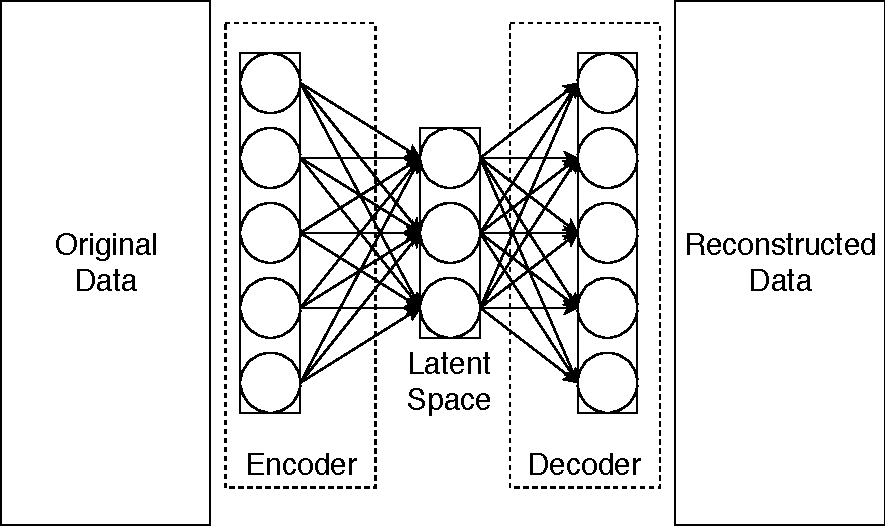
\includegraphics{figs/Autoencoder.pdf}
\caption{Example of a single layer autoencoder.
In this case, both the encoder and the decoder are a single layer neural network.
These layers can be stacked to create even more complex dimensionality reductions.}
\end{center}
\label{fig:ae}
\end{figure}

The implementation of autoencoders usually uses neural network layers to learn the encoding and decoding functions.
Figure \ref{fig:ae} demonstrates an example structure of a very simple autoencoder.
There are a number of different types of autoencoders that are extensions of this basic idea.
One example is a sparse autoencoder.
In order to force the autoencoder to learn a more general dimensionality reduction, we can add a sparsity constraint to limit the number of activations among the network layers.
This forces the autoencoder to learn a representation with sparse network weights.
Another type of autoencoder is a denoising autoencoder.
This type of autoencoder involves taking a noisy representation and mapping it back to a clean representation of the data.
This can either be trained on noisy data or it can be given the original representation, corrupt it, and then try to learn the original representation from the corrupted data.

Sometimes we want to do more than just learn arbitrary encoding and decoding functions.
For instance, we might want to impose constraints on the encoded representation, also known as the latent space.
\glspl{vae} are a class of autoencoder that does exactly this.
\glspl{vae} constrain the encoded representation to be a probability distribution.
So, instead of learning functions that encode/decode the data, the \gls{vae} actually learns the parameters of the encoded probability distribution.
Specifically, the encoder learns to map samples to a mean and standard deviation, which is our latent space.
Then, when decoding the sample, we can sample randomly using the encoded mean and standard deviation as parameters for our probability distribution.

We measure loss in this scheme through a combination of two loss terms.
First, we still care about how well we are able to reconstruct our original data.
So, we can have a reconstruction loss term which measures how well the reconstructed data maps to the original data.
Our second loss term constrains the latent space to ensure that it is well formed and provides a regularization term against overfitting.
We use \gls{kl} divergence, a common way of measuring difference between probability distributions.
We can calculate the the \gls{kl} divergence between our latent space and our prior distribution, which in most cases is a normal distribution.
With the combination of those two loss terms, we can then train the \gls{vae} as we would any other neural network---by using gradient descent to minimize the loss function.

We denote $x_i \in X$ as our data and $z$ as our latent representation.
Our encoder network can be represented by the function $p$ which has parameters $\theta$.
Similarly, our decoder can be represented as a posterior distribution $q$ that is parameterized by $\phi$.
Then the loss function of a \gls{vae} can therefore be written out as follows:

\begin{equation}\label{eqn:vae-loss}
\mathcal{L}(\theta, \phi) = - E[\log p_{\theta}(x_i | z)] + KL(q_{\phi}(z | x_i) || p(z)) \\
\end{equation}

%TODO: add here

\chapter{Related Work} \label{chap:rw}
This chapter introduces related work in the relevant fields of computer science and biological modeling.
In particular, we examine work in the field of building metabolic models using flux balance analysis.
Next, we present a series of automatic reduction systems for metabolic models.
None of these systems have been applied to modeling cell-free systems, though we present other versions of models.
Finally, we investigate recent work in the field of variational autoencoders.

%FOCUS ON BIOLOGISTS/USABILITY

\section{Flux Balance Analysis}
Early metabolic models in the 1980s pioneered the use of stoichiometric equations to describe a biological system and predict the yield of a specific product~\cite{papoutsakis1984equations}.
This work was soon improved through the use of linear programming (\gls{lp}) to solve for the optimal result~\cite{fell1986fat}.
After the transition to using \gls{lp} solvers, this field was referred to as constraint based analysis, while the primary technique used to solve these equations is called \gls{fba}.
These techniques were soon applied to describe the main metabolic systems in \gls{ecoli}~\cite{majewski1990simple}.
Importantly, \gls{fba} has repeatedly been shown to predict phenotypes that corresponded to real-world data~\cite{varma1994stoichiometric, edwards2001silico, segre2002analysis, bordbar2014constraint}.

Improvements on these early models have primarily included the addition of new genes, metabolites, and reactions~\cite{varma1993metabolic}.
In particular, after the first \gls{ecoli} genome was sequenced and annotated, the size of these models grew rapidly.
The earliest genome scale model (\gls{gem}) for \gls{ecoli} was iJE660a, a model that accounted for 627 unique reactions in a typical \gls{ecoli} cell~\cite{edwards2000escherichia}.
Over the years, more and more reactions were progressively added to the model to better describe the biology.
This work will use the most recent \gls{ecoli} \gls{gem}, iJO1366 from 2011, which contains 2583 reactions~\cite{orth2011comprehensive}.
Since 2011, work in this field has focused on extending metabolic models to incorporate more biological information.
For instance, recent work has involved the addition of gene expression data to create metabolism and gene expression models (\glspl{me})~\cite{lloyd2017cobrame}.
The most recent \gls{me}, iJL1678-ME has 79871 reactions.

%There has also been a sizable amount of research done on extensions to \gls{fba}.
%People have added thermodynamic constains 

\section{Reduction of metabolic models}
As these \glspl{gem} begin to incorporate even more information, the issue of high dimensionality arises.
%One issue with using a full \gls{gem} is the extremely high dimensionality due to the fact that every reaction occurring in a cell is detailed.
To deal with this issue, a number of papers have tried to reduced these genome scale models to only the most essential reactions.
One group has developed multiple tools to reduce the dimensionality of these models.
red\gls{gem} performs a graph search with the objective to minimize information loss to find core metabolic models~\cite{ataman2017redgem}.
Similarly, lumpGem identifies and collapses reaction networks into single balanced reactions in order to reduce the overall dimensionality of the model~\cite{ataman2017lumpgem}.
The other major tools in this area are NetworkReducer and minNW.
NetworkReducer iteratively prunes and compresses reaction networks while maintaining a set of protected reactions until a core model is found~\cite{erdrich2015algorithm}.
minNW uses mixed-integer linear programming (\gls{milp}) techniques to compute minimal subnetworks with certain constraints~\cite{rohl2017mixed}.

All of these methods are searching for minimal core models using only the stoichiometric description of the system.
However, there has also been work that uses general dimensionality reduction techniques such as Principal Component Analysis (\gls{pca}).
This idea was incorporated into a search technique called Principal Element Mode Analysis (\gls{pema})~\cite{von2016principal}.
\gls{pema} searches for subnetworks that maximize the observed variance similar to how the principal components of \gls{pca} work.
More recent methodology called "Principal metabolic flux mode analysis" explicitly incorporates \gls{pca} and \gls{fba}~\cite{bhadra2017principal}.
They reduce the dimensionality of the system by running \gls{pca} on the stoichiometric matrix while using the concepts from \gls{fba} as regularization.
%Bayesian \gls{fba}
%Network models on \gls{fba}

%TODO: Fix up paragraph
We differ from earlier reduction techniques in a few ways.
Firstly, none of these techniques have incorporated deep learning methods.
In addition, these techniques all deal with the stoichiometric matrix in the abstract without having actual experimental data to learn from.
Finally, none of the techniques above have specifically targeted \gls{cfps} systems.

\section{Modeling cell-free systems}\label{rw:mod-cf}
Models of cell-free systems have typically been based on kinetic models of transcription and translation.
These models have a narrow focus because they only examine reactions involved in transcription and translation.
Those reactions can then be described using differential equations with known rate constants to describe the rate of transcription and translation.
This type of model has been applied to the commercial \gls{ecoli} cell-free system TXTL, and was able to accurately describe the dynamics of their gene circuit of interest~\cite{tuza2013silico}.
Other work has proposed a general framework to model metabolic networks in cell-free systems using these kinetic models~\cite{wayman2015dynamic}.
Even more recent work in this field includes using Bayesian parameter inference to infer the kinetic parameters for these reactions in less well studied organisms~\cite{moore2018rapid}.

There have only been a few attempts to use metabolic models and \gls{fba} to model cell-free systems.
One model attempted to adapt a full-scale \gls{ecoli} model to a cell-free system by hand~\cite{bujara2012silico}.
The authors decided which parts of the full model were relevant for cell-free systems and then removed any irrelevant reactions from the model.
A more recent attempt took a bottom-up approach to building a \gls{fba} model for cell-free systems~\cite{vilkhovoy2017sequence}.
Instead of removing reactions from the full \gls{ecoli} \gls{gem} until they had a cell-free model, the authors instead selected a few pathways they felt were crucial for a cell-free system.
They then built a model using only the reactions they had selected as important for protein synthesis.
%Importantly, their model is 'sequence specific', meaning it is tailored to the specific gene product of the cell-free system.
These models show that it is possible to use \gls{fba} to describe cell-free systems,.
However, neither approach is able to construct cell-free systems in a systematic way that could scale to other labs or other organisms.

%Hybrid agent-based model for quantitative in-silico cell-free protein synthesis. 2016
%https://www.ncbi.nlm.nih.gov/pmc/articles/PMC5288458/

\section{Variational autoencoders}
Autoencoders have been around for many years, but \glspl{vae} were first introduced only in 2014~\cite{kingma2013auto, rezende2014stochastic}.
Since their introduction, \glspl{vae} have been used for everything from transferring image features~\cite{larsen2015autoencoding} to molecule generation~\cite{gomez2016automatic}.
Due to their ability to function as generative networks, much of the work in the field has focused on applying \glspl{vae} to images.
\glspl{vae} have only just begun making their way into analyzing biological data.
Recent work includes using a \gls{vae} on cancer transcriptomics data to extract meaningful features of cancer gene expression~\cite{way2017extracting}.

%Also introduced by ~\cite{rezende2014stochastic}
Work has also been done to incorporate correlation terms with \glspl{ae}.
Correlation Neural Networks were first introduced as a way to make \glspl{ae} more effective on multi-modal data such as labeled images~\cite{chandar2016correlational}.
By maximizing the correlation between the latent representations for each view of the data, the authors were able to improve performance.
This idea has been expanded in Relational Neural Networks, which also looks at correlation within the data to affect the \gls{ae} loss term~\cite{meng2017relational}.

\chapter{Design and Implementation} \label{chap:impl}

<<<<<<< HEAD
=======
%FOCUS ON BIOLOGISTS/USABILITY

>>>>>>> d36f4c58ce53756c4208d542755ca45e64177c23
The primary deliverable of this dissertation is a system, \gls{sys} (shown in Figure \ref{fig:overview}) that is able to generate metabolic models of cell-free systems.
This chapter decomposes \gls{sys} into its four main parts.
First, \gls{sys} ingests experimental data and converts it into a standardized format.
Next, \gls{sys} uses the data to construct a group of cellular metabolic models and sample fluxes from those models to create a dataset.
Then, \gls{sys} performs dimensionality reduction to elucidate underlying trends in the experimental data.
Finally, \gls{sys} leverages those insights to reduce the original, overspecified models to standalone cell-free metabolic models.

\section{Data gathering}
In order to build a robust model that reflects biological reality, I first had to generate data to use for training.
Gathering high quality biological data is difficult and is crucial to the success of the system as a whole.
I describe the high level process of creating a cell-free system and running the experiments below.
The full experimental protocol can be found at dx.doi.org/10.17504/protocols.io.kz2cx8e.

\begin{figure}[t!]
\begin{center}
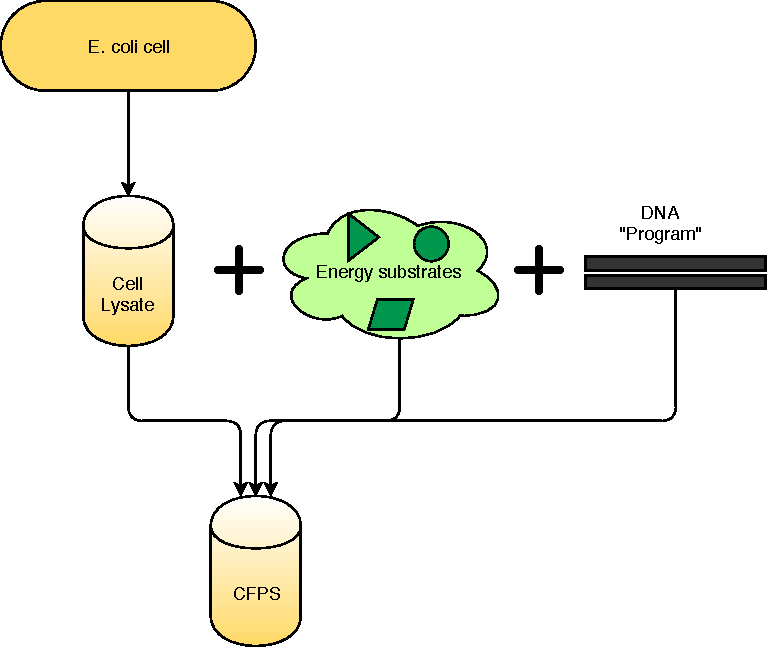
\includegraphics{figs/CellFreeSetup.pdf}
\caption[Process for creating a \gls{cfps} system]{Process for creating a \gls{cfps} system.
The \gls{ecoli} cells can be grown up in bulk, allowing future preparation of \gls{cfps} reactions to be far quicker than typical \textit{in vivo} methods.
}
\end{center}
\label{fig:cfps}
\end{figure}

\subsection{Cell-free systems}
As shown in Figure \ref{fig:cfps}, creating a cell-free protein expression system involves three main steps: growing and lysing cells, supplementing with energy substrates, and adding custom \gls{dna} constructs.
This protocol is based on an open protocol from the Federici lab \cite{medina2017cfps}.
I began by growing up 1L of BL21 \gls{ecoli} cells in an overnight culture of \gls{lb} until they reached an \gls{od} of 1.6.
The cells were then split into 45 \gls{ml} aliquots centrifuged for 12 minutes at 4500\textit{g}~and the supernatant is poured off.
The pellet was then be stored in a 4\degree~refrigerator overnight if necessary.
Next, the cells underwent 2 more sets of centrifugation with the same settings; the pellet was resuspended each time with 45 \gls{ml} of S30A buffer (see Appendix \ref{app:exp} for buffer compositions).
The cells were then centrifuged twice more at 2000\textit{g}~ for 8 and 2 minutes.
In between the final two centrifugations, the cells were resuspended with 37.5 \gls{ml} of S30B buffer.
After the final centrifugation step, the pellets were weighed and resuspended with $0.9$ times their weight in S30A and $5$ times their weight of $0.1$ mm beads.
Using a bead beater set to 46 rpm, the cells were beaten for 30 seconds, rested on ice for 1 minute, and then beaten for another 30 seconds.
These lysed cells were spun one final time for 8 minutes at 4500\textit{g}~to remove the cellular debris and beads.
The supernatant was then removed as a cell extract and stored in a -80\degree~freezer.

This cell extract contains the core cellular machinery that is necessary for transcription and translation.
However, the full \gls{cfps} system requires additional reactants that are important for the transcription and translation reactions.
The addition of these reactants to the cell extract creates a full \gls{cfps} system.
These substrates include cofactors such as \gls{camp}, maltodextrin, and \gls{nad}, as well as vital building blocks of transcription and translation such as \glspl{ntp}, \glspl{aa}, and \glspl{trna}.
Table \ref{tab:cf-nrg} lists each of the reactants and their purpose in the cell-free system, while Table \ref{tab:cf-conc} shows the final concentration for each reactant.

This cell-free expression system acts a biological computer.
Whatever \gls{dna} ``program" is added, the system will work to produce the appropriate protein result.
This platform is powerful because it allows a user to easily insert these \gls{dna} programs and see results within a few hours.
A typical biological timeline would take far longer because living cells would have to be transformed (a lengthy process) to uptake the \gls{dna} and incorporate it into their production processes.

\begin{table}[]
\centering
\begin{tabular}{lll}
\textbf{Reactant }    & \textbf{Amount} (\gls{ul}) & \textbf{Purpose}                        \\
Maltodextrin solution          & 5               & Energy substrates               \\
Amino acids         & 10              & Building blocks for \gls{tl} \\
\gls{peg}          & 2.5             & Molecular crowding              \\
\gls{hmp}          & 1               & Phosphate source                \\
\gls{mg}           & 0.74            & Important cofactor              \\
\gls{k}            & 0.8             & Charge homeostasis              \\
\gls{dna}          & 0.8             & Template for protein   \\
Cell extract & 25              & \gls{tx}/\gls{tl} machinery                 \\ \hline
\gls{cfps} system        & 50              & Protein production             
\end{tabular}
\caption[List of reactants for a 50 \gls{ul} \gls{cfps} reaction]{List of reactants for a 50 \gls{ul} \gls{cfps} reaction. 
See the final concentrations of all reactants in Table \ref{tab:cf-conc}.
Note that MDX is a mixture of substrates (also detailed in Table \ref{tab:cf-conc}).
Amino acids includes all 20 of the amino acids.
}
\label{tab:cf-nrg}
\end{table}

\begin{table}[]
\centering
\begin{tabular}{llll | l}
Sugar & \gls{hmp} & \Glspl{ntp} & \gls{k} & Normalized output   \\ \hline
0    & 0    & 1    & 0    & 0.57 \\
0    & 1    & 0    & 0    & 0.52 \\
1    & 0    & 0    & 0    & 0.59 \\
0    & 0.5  & 0.5  & 0    & 0.97 \\
0.5  & 0    & 0.5  & 0    & 0.76 \\
0.5  & 0.5  & 0    & 0    & 0.20 \\
0.25 & 0.25 & 0.5  & 0    & 0.40 \\
0.25 & 0.5  & 0.25 & 0    & 1.00 \\
0.5  & 0.25 & 0.25 & 0    & 0.96 \\
0.25 & 0.25 & 0.25 & 0.25 & 0.36 \\
0    & 0    & 0    & 1    & 0.19 \\
0    & 0    & 0.5  & 0.5  & 0.22 \\
0    & 0.5  & 0    & 0.5  & 0.16 \\
0.5  & 0    & 0    & 0.5  & 0.16 \\
0    & 0.25 & 0.25 & 0.5  & 0.37 \\
0.25 & 0    & 0.25 & 0.5  & 0.47 \\
0    & 0.5  & 0.25 & 0.25 & 0.26
\end{tabular}
\caption[Different reaction concentrations for our Manual dataset]{Different reaction concentrations for our Manual dataset.
Reactant columns are measured in \gls{ul}, while the output column has been normalized by the maximum level of fluorescence observed.
Each experiment was repeated $n = 2$ times at a total volume of 6\gls{ul}.
}
\label{tab:manual}
\end{table}

\subsection{Datasets}
The protocol above was used to create two datasets for training.
The first dataset was created by hand and followed standard lab procedures.
Each of the reactants specified by Table \ref{tab:cf-nrg} was combined in the appropriate ratio to create a 200 \gls{ul} mastermix. 
That mastermix was then split into 5 \gls{ul} aliquots.
1 \gls{ul} of varying concentrations of the energetic substrates were added to each aliquot, bringing the total reaction volume to 6 \gls{ul} .
This dataset is composed of 17 differing ratios of sugar, phosphate, potassium, and nucleotides.
I used a \gls{dna} circuit that encodes the \gls{rfp} gene, so the amount of protein production was measured using fluorescence readout with a plate reader.
The results for those reactions are shown in Table \ref{tab:manual}

One of the downsides to generating this data by hand is that creating large datasets by hand takes a long time.
To increase the amount of data generated, I created a second dataset using a Labcyte Echo acoustic liquid handler.
The Echo is an acoustic liquid handler that can programmed to combine different amounts of liquid.
Using the Echo, I was able to generate a larger number of different experimental conditions for the \gls{cfps} reactions.
Additionally, pipetting by hand has intrinsic error, while the Echo is able to transfer liquids in multiples of 2.5 \gls{nl} with less than 2\% error.
The Echo therefore has the dual benefits of generating more data and reducing the amount of noise in that data.
The experiments on the Echo were performed using 2\gls{ul} of \gls{cfps} system and 500 \gls{nl} of additional reactants.
The use of automation allowed us to test 51 different reaction conditions and shows that this could be expanded to an even larger scale.

Finally, I also used a third dataset from the recent Karim and Jewett paper that uses \gls{cfps} systems to perform metabolic engineering~\cite{karim2018controlling}.
Their protocol is very similar to the one I showed above, though the final composition of the reactants differs.
This dataset is useful because it was created in a different lab and they measured the output using liquid chromatography, not fluorescence.
Since this dataset was created in different lab conditions, it can be used to check that our system is generalizable to cell-free systems as a whole and not just overfitting data generated from my \gls{cfps} system.

We will refer to these datasets as our "Manual", "Echo", and "Karim" datasets.

\begin{figure}[t!]
\begin{center}
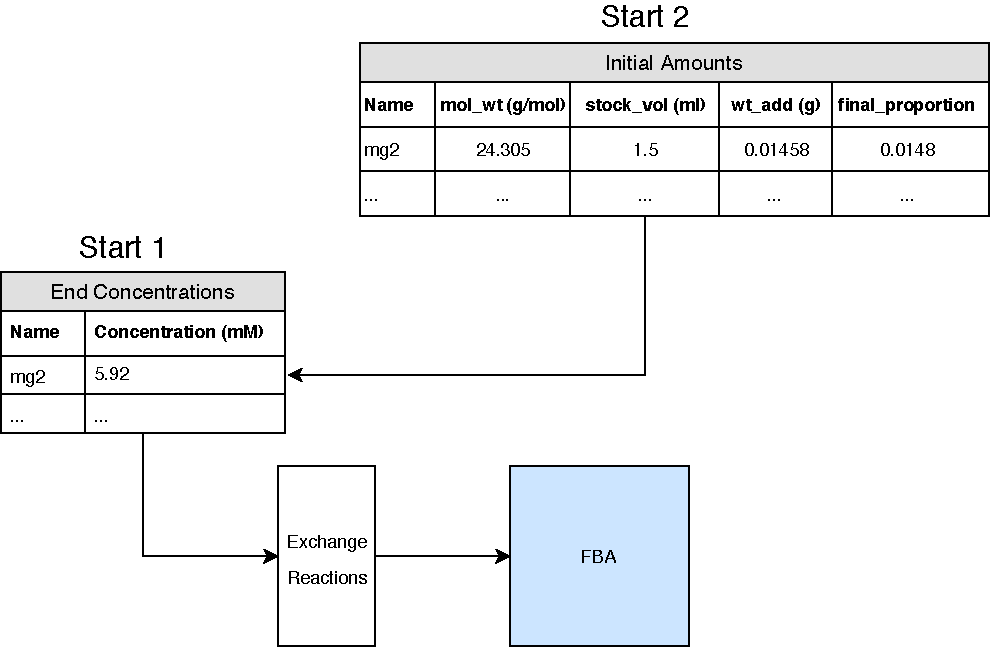
\includegraphics[width=\textwidth]{figs/DataIngestion.pdf}
\caption[Data ingestion part of \gls{sys}]{Two possible ways to incorporate the experimental setup in \gls{sys}.
In Start 1, the user already knows the final concentrations of each reactant and can upload that as a \gls{csv}.
Otherwise, the user can upload information about the reactants that are added and our tools will automatically calculate the final concnetrations of each reactant.}
\label{fig:ingest}
\end{center}
\end{figure}

\section{Data ingestion and incorporation}

\subsection{Data ingestion}
Since this system is intended to aid biologists in their experiments, I designed it to be usable without any coding experience.
With that in mind, I created two separate ways to incorporate the experimental setup into the models.
Figure \ref{fig:ingest} shows the acceptable structures of the experimental setup .
The first structure is a \gls{csv} containing the final concentrations of the different reactants in the cell-free system.
This is the easiest to incorporate because it is a simple conversion from concentrations to fluxes.
Fluxes have the unit mol/min/gDW, so they can be converted from metabolite concentrations into fluxes using the following equation from MetaboTools~\cite{aurich2016metabotools}:
\begin{equation}
f = \frac{m}{c * t * 1000.0}
\end{equation}
where $f$ is the flux value, $m$ is the concentration of our metabolite, and $c$ is the overall concentration of the cell.
I used $t = 24$ because our reactions ran for 24 hours.
Using this equation, \gls{sys} is able to ingest a \gls{csv} mapping the name of the reactant to the final concentration and turn them into flux constraints.

However, \gls{sys} also supports users who might only know the relative amounts of each reactant that they are adding, but not the final concentrations of their reactants.
This is important because many biologists may have a protocol that they follow that tells them how to make a \gls{cfps} system, but they may not know the final concentrations in their mixture.
\gls{sys} allows those users to use a \gls{csv} (or combination of \glspl{csv}) that contains information about each reactant used to make the system.
Each row has the name of the reactant, its molecular weight, the weight used to create the stock, the volume used to create the stock, and the final volume of the stock added to the cell-free reaction.
Using this information, \gls{sys} calculates the final concentration of each reactant in the \gls{cfps} system and converts it to the same form as the other branch of the pipeline.
Once the data is in its canonical form of final concentrations, \gls{sys} proceeds with the a unified computational pipeline.

\subsection{Data Incorporation} \label{sec:incorp}
After ingesting the experimental setup, \gls{sys} incorporates it into a \gls{fba} model.
The \gls{fba} models are handled via the \gls{cobra}py python package~\cite{ebrahim2013cobrapy}.
\gls{sys} uses the iJO1366 model for its base model of \gls{ecoli}.
iJO1366 consists of 1805 metabolites and 2583 reactions~\cite{orth2011comprehensive}.
This model describes \gls{ecoli} cells, and needs to be adapted to cell-free systems because they no longer have the same physical structure as \gls{ecoli} cells.
First, \gls{sys} changes every reaction reflect the fact that there are no longer any membranes or cellular compartments.
Every reaction that contains a periplasmic or extracellular component is moved into the cytosol.
This is handled by replacing every metabolite in the model with its corresponding cytosolic version.
If no corresponding cytosolic metabolite exists, \gls{sys} creates a cytosolic version of the metabolic and then proceeds as above.
After this step, all of the reactions in the model occurring in the same compartment, which reflects how a \gls{cfps} system works.

\gls{sys} then handles the specific experimental data that was earlier ingested through the use of exchange reactions.
Exchange reactions are pseudo-reactions that allow a \gls{fba} model to constrain the amount of a reactant present in the model.
For each of the reactants in a \gls{cfps} system, \gls{sys} creates an exchange reactions with bounds based on the fluxes that were calculated earlier.
At the end of this process, \gls{sys} has converted the full-scale \gls{ecoli} model to better approximate a \gls{cfps} system.
This type of model has not been generated before, but it is still overspecified.
This model is what is later used to reduce into a base cell-free model.

\gls{sys} also provides the option to explicitly incorporate the transcription and translation reactions that are so crucial to \gls{cfps} systems.
Most \gls{fba} models do not explicitly model the transcription and translation reactions.
However, earlier work from the Varner lab incorporated these reactions into a \gls{fba} model specifically to try to model a cell-free system~\cite{vilkhovoy2017sequence}.
This earlier work created the \gls{fba} model by hand and is written in Julia.
\gls{sys} provides auxiliary tools to, given the sequence of the gene of interest, automatically generate a relevant version of the Varner model.
That model is converted to Python and the relevant transcription and translation reactions are extracted.
Those reactions are then incorporated into the base cell-free model, creating a TXTL cell-free model.
<<<<<<< HEAD
=======

%As a linear programming problem, we also need to set a custom objective to optimize for.
%Usually this is the biomass objective, which encapsulates everything necessary for bacterial growth.
%However, since we don't care about growth, just production, we can use our own objectives.
%For us, the typical objective will be the production of some protein since that's the purpose of the \gls{cfps}.
>>>>>>> d36f4c58ce53756c4208d542755ca45e64177c23

\section{Dataset generation}

\subsection{Model generation}
Once \gls{sys} has created these base models, it uses them to create a different model for each experimental condition.
\gls{sys} reads in a \gls{csv} consisting of the experimental conditions and a quantitative output.
Each row represents a different experiment and each column contains the amount of additional reactant that was added.
\gls{sys} then re-calculates the final concentrations of each of the reactants for each experimental starting condition.
Those new concentrations are used to update the constraints for the exchange reactions of each reactant.
For each unique experimental condition, \gls{sys} creates a new \gls{fba} model.

These experimental condition models are still overspecified and therefore have the same optimal solution.
Thus, these naive models poorly describe the biological reality of the datasets (see Section \ref{sec:cmp} for a comparison).
Clearly, \gls{fba} does not describe what is occurring in a \gls{cfps} system.
These \gls{fba} models contain every reaction that is occurring in a steady state bacterium.
While the bacteria are harvested at steady state, not all reactions will maintain their importance in a cell-free system.
I hypothesized that these base models failed to describe cell-free systems because the differences between a cell-based system and a cell-free system cannot be encapsulated solely through different exchange reactions and the creation of a single-compartment system.

\gls{fba} acts as a coarse, non-linear amplifier, so points that vary only slightly in the input parameter space may not differ very much in the output space.
I wanted to improve the granularity of \gls{fba} response by passing the fluxes through a dimensionality reduction technique such as a \gls{vae}.
In order to do this, I needed a large dataset of fluxes to train on.
Although the experimental conditions led to only have a small number of models, I was able to create large datasets by flux sampling from each model.

\begin{figure}[t!]
\begin{center}
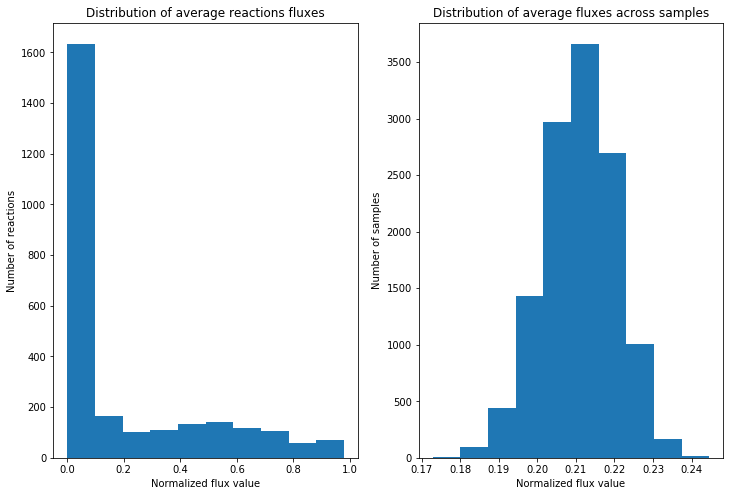
\includegraphics[width=\textwidth]{figs/fluxdistribution.png}
\caption[Distribution of fluxes generated by flux sampling]{Distribution of fluxes generated by flux sampling.
X axes represent the value of the fluxes and have been scaled to between 0 and 1.
The plot on the left shows a histogram of the average flux value for each reaction.
Most reactions have an average flux that is close to 0.
The right plot shows the average flux across samples.
The average flux across all samples clusters around 0.21. 
}
\label{fig:distrib}
\end{center}
\end{figure}

\subsection{Flux sampling}
Flux sampling is the process of sampling possible fluxes through each reaction.
\gls{sys} performs flux sampling on each model of a different experimental condition.
For each model, this generates a distribution of fluxes for every reaction in that model.
Figure \ref{fig:distrib} shows the average distribution of fluxes for each sample and each reaction.
Flux sampling is implemented using the optGpSampler routine~\cite{megchelenbrink2014optgpsampler}.

Each model has different experimental conditions and therefore has slightly different flux distributions for each reaction.
So, after generating flux samples for each model, these sampled fluxes are combined to generate two new datasets.
One dataset is flat---meaning we simply concatenate all of the sampled fluxes into a single dataset.
This dataset has size $(N * E) \times R$ where $N$ is the number of samples, $E$ is the number of experiments, and $R$ is the number of reactions.
This flat dataset is useful to investigate the fluxes using typical dimensionality reduction techniques.
However, \gls{sys} also generates a stacked dataset of size $N \times E \times R$. 
This involves sampling with replacement from the distribution of fluxes of each model and then stacking the fluxes to create a new dataset.
Using this version of the dataset facilitates the training of a Corr-VAE.
I used this part of \gls{sys} to generate flat and stacked versions of all three of the datasets described above.

\section{\gls{vae}} \label{sec:vae}
As mentioned earlier, the base cell-free \gls{fba} models did not describe our experimental data well.
To solve that issue, \gls{sys} implements a \gls{vae} to reduce the dimensionality of our models.
The \gls{vae} is implemented using the Keras framework~\cite{chollet2015keras} and the implementation was designed to be as modular as possible.
Because the Corr-VAE has applications in other parts of biology, I implemented all \glspl{vae} to make it easy to change their parameters.
Thus, my implementation takes in command-line arguments to specify either a flat or stacked dataset, a list of layer sizes, the number of latent dimensions, how to scale the inputs, and whether or not to use the custom correlation loss function.
I also provide sensible default values for those users who have less experience in the field of deep learning.

The structure of the \glspl{vae} we used are as follows.
I experimented with two different layer structures, a 2-layer \gls{vae} with layer sizes 1024 and 256 and a 3-layer \gls{vae} with layer sizes 1024, 1024, and 1024.
The 3-layer \gls{vae} performed much better, so that was the structure I used for all subsequent experiments.
I also tried using latent dimensions of size 2 and 10.
Both 2 and 10 dimensions are able to capture relevant information in their latent space, though future work could use even more latent dimensions.
Activations between layers of both the encoder and the decoder were \glspl{relu}~\cite{nair2010rectified}.
The final layer of the \gls{vae} used a sigmoidal activation to produce scaled fluxes between 0 and 1.

\subsection{Corr-VAE}
Placing a regular \gls{vae} on top of a \gls{fba} model will simply attempt to reconstruct the fluxes.
However, I did not just want to reconstruct fluxes in an unbiased way---I wanted the reconstructed fluxes to correspond to the real-world biological data.
The key insight of a Corr-VAE is that the experimental data can be used to perturb the latent space to better reflect biological reality.
A Corr-VAE incorporates the experimentally determined output values into its loss function.
It does so by adding a loss term consisting of the correlation between the experimental data and the reconstructed flux that represents the objective function.
Recall Equation \ref{eqn:vae-loss} that described the normal \gls{vae} loss function.
The Corr-VAE loss function is now written as:

\begin{equation}\label{eqn:corr-loss}
\mathcal{L}(\theta, \phi) = - E[\log p_{\theta}(x_i | z)] + KL(q_{\phi}(z | x_i) || p(z)) + corr(x_i', d)\\
\end{equation}

where $x_i'$ is the reconstructed data, $d$ is the experimentally determined biological data, and $corr$ is the Pearson correlation between the two.
I also experimented with weighting the correlation loss term to force the representation to be closer to the real world data, but this did not appear to have a large effect.
Corr-VAEs required a stacked dataset in order to calculate the correlation between the experimental data and the output fluxes.
By default \gls{sys} uses a Corr-VAE to reduce the dimensionality of a generated dataset.

\section{\gls{fba} model reduction}
The Corr-VAE is able to generate a lower dimensional representation of the base cell-free models.
\gls{sys} uses the reconstructed representation to create better cell-free models.
After examining the latent space of the Corr-VAE to ensure that it was learning the differences between the models, I was able to use the reconstructed fluxes to reduce the original models.
For each experimental condition model, \gls{sys} uses the reconstructed fluxes from the Corr-VAE to determine which reactions are unimportant.
It does this by creating a threshold and removing any reactions that have a flux under that threshold.
By doing this for each model, it builds up a list of reactions that are not used in any of the experimental models.

\gls{sys} then uses removes all of those reactions from the base model to generate a new cell-free model.
The value of this model is tested by comparing how well the optimal fluxes correlate with the experimental data.
Section \ref{sec:cmp} shows that these reduced models with the differential conditions give us better explanations of experimental data than full \glspl{gem}.
The thresholding is a simple method of identifying which reactions are not important in cell-free systems.
Future work could generate improved reduced models by using more sophisticated reduction techniques in conjunction with the Corr-VAE.

\chapter{Results}\label{chap:res}

\section{Comparison of models}

\section{Emphasis on where FBA-VAE does particularly well}

\section{Noise addition}

\section{Transfer learning}

\section{Biological insights}

\chapter{Future Work} \label{chap:fw}

\section{Further datasets}
The datasets that used in this dissertation are relatively small---on the order of 10s of different parameter combinations.
The limited scope of these datasets means that they are only able to coarsely cover the entire parameter space.
I hypothesize that one way to get better reduced models would be to train using data generated from more of the parameter space.
Generating large biological datasets by hand is difficult and error prone.
However, this dissertation demonstrated the potential for further lab automation by generating a dataset using the Labcyte Echo liquid handler.
Future work will take this even further and generate datasets with hundreds or even thousands of starting conditions.
Another logical extension is to use datasets generated from organisms other than \gls{ecoli}.

\begin{figure}[t!]
\begin{center}
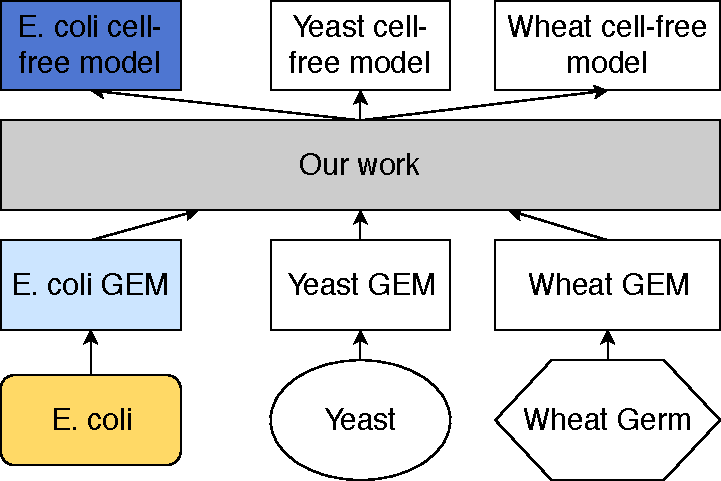
\includegraphics{figs/Vision.pdf}
\caption[\gls{sys} can generate cell-free models for any organism]
{\gls{sys} was designed to convert any organism's \glspl{gem} into an appropriate cell-free model.
}
\end{center}
\label{fig:vision}
\end{figure}

\section{Different Organisms}
This work has only explored the generation of \gls{ecoli} cell-free models.
However, much ongoing work involves the use of non-\gls{ecoli} organisms.
This system was written in such a way that it can be applied to any organism with a \gls{gem}.
Figure \ref{fig:vision} demonstrates one potential vision of how \gls{sys} could be used in the future.
Instead of creating a model by hand that only describes our \gls{cfps} system, \gls{sys} can be used to create cell-free metabolic models for many different organisms.
In particular, I am also a part of an OpenPlant grant involving modeling wheat-germ cell-free systems.
The data is currently being generated, and I plan to apply \gls{sys} to this new \gls{cfps} system as soon possible.

\section{RL system for reduction}
The use of a \gls{vae} as a dimensionality reduction tool proved to be quite powerful, but the part of the system that converted from the reduced representation back into a \gls{fba} model was quite simple.
\gls{sys} removes reactions based on a simple thresholding criterion.
Instead of deciding which reactions to remove using a threshold, future version of \gls{sys} could reframe this problem as a reinforcement learning problem.
Using a combination of experimental data, a starting \gls{fba} model, and a latent representation of the problem space, these more sophisticated search methods could likely produce better reduced models.
To that end, I have also built a framework on top of OpenAI's Gym environment for performing reinforcement learning on \gls{fba} models.
Given a starting model with almost 2600 reactions, the search space of possible reduced models is enormous.
However, a combination of the Corr-VAE and reinforcement learning could perform a targeted search and yield a better reduced model.

\begin{figure}[t!]
\begin{center}
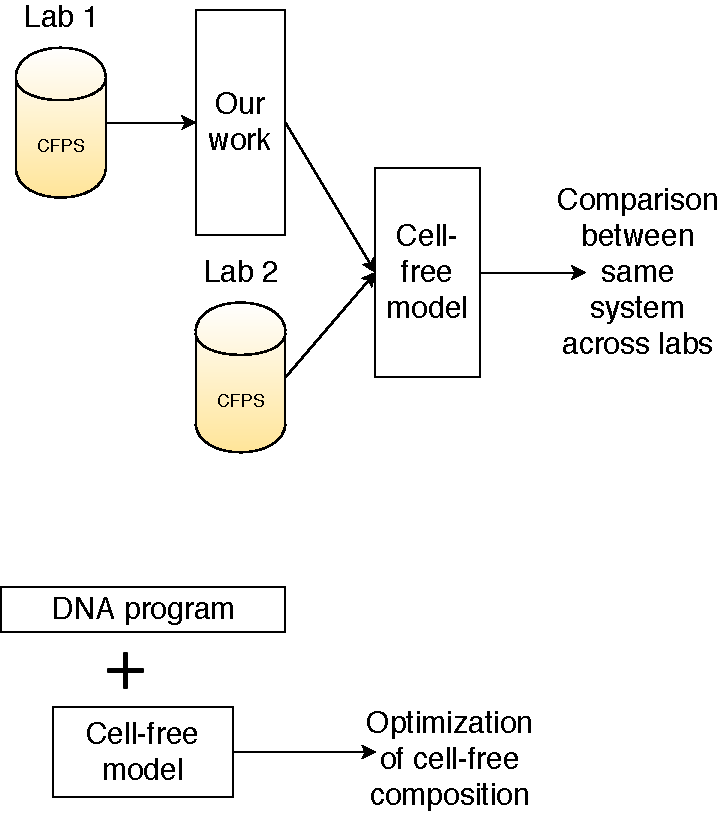
\includegraphics{figs/Applications.pdf}
\caption[Future applications of \gls{sys}]
{Two future applications of \gls{sys}.
Above, multiple experiments can be projected in the same subspace to better compare experimental results.
Below, the system can help optimize the energetic composition of a cell-free system}
\end{center}
\label{fig:apps}
\end{figure}

\section{Batch variation}
Finally, an important use case for \gls{sys} is as a way to deal with batch variation in \gls{cfps} systems.
Batch variation is an important problem facing the cell-free community~\cite{sun2013protocols, chizzolini2017cell}.
The current solution to this problem is to run everything that needs to be compared in the same batch.
This is problematic, though, if the batch runs out or someone else wants to reproduce this result.
The only way to deal with this problem would be to redo all of the experiments in a new batch.

Figure \ref{fig:apps} demonstrates how \gls{sys} provides a potential solution to this issue of batch variation.
A researcher runs a calibration set of experiments and then uses those experimental results to generate a \gls{vae} model.
Now, this \gls{vae} can be used to project any future experimental data into the same latent space as the first set of experiments.
These experiments could be compared within the latent space, or they could be transformed back into the original dimensionality of the data and then compared.
This transformed data should allow for better comparisons across batches.

\chapter{Conclusion}

%TODO: fix conclusion
In conclusion, we have shown that deep learning techniques can be successfully applied to biology.
In particular, computational biologists should start using \glspl{ae} (especially \glspl{vae}) for dimensionality reduction instead of defaulting to using \gls{pca}.
Among our contributions are the new loss function that we developed for our \gls{vae}, which is general enough to be used with any biological data and the set of new \gls{ecoli} \gls{cfps} metabolic models.
We hope this work encourages other computational biologists to continue work integrating deep learning with biology in general and metabolic models specifically.

%\appendix
%\chapter{Experimental Setup}\label{app:exp}
\appendix
\chapter{Experimental Setup}
\label{app:exp}

\section{Buffers}
To create S30A buffer, combine 10.88g Mg-glutamate, 24.39g mM K-glutamate, 50 mL Tris and titrate with acetic acid to reach pH 7.7.
Add water to 2L and autoclave.
Before using, add 4 ml of 1 M DTT.

For S30B buffer, combine 10.88g mM Mg-glutamate, 24.39g mM K-glutamate, and titrate with 2M Tris until pH 8.2.
Add water to 2L and autoclave.
Add 2 ml of 1 M DTT before using.

\section{Supplementary Tables}

\begin{table}[h!]
\centering
\begin{tabular}{ll}
Compound     & Concentration (\gls{mm}) \\ \hline
\gls{hmp}           & 0.981              \\
\gls{mg}           & 5.92               \\
\gls{k}           & 48.0               \\
\gls{nad}          & 0.454              \\
\gls{coa}          & 0.353              \\
\gls{camp}         & 1.01               \\
Folinic acid & 0.092              \\
Spermidine   & 0.181              \\
Glucose      & 5.42               \\
ATP/GTP      & 2.09               \\
CTP/UTP      & 1.26               \\
\glspl{aa}  & 35.6               \\
\gls{trna}        & 0.010              \\
\gls{dna}          & 0.071             
\end{tabular}
\caption{Final concentrations of reactants in our \gls{cfps} reaction}
\label{tab:cf-conc}
\end{table}

\begin{longtable}{lll | l}
%\begin{tabular}
Sugar & \glspl{aa} & \glspl{ntp} & Normalized output   \\ \hline
0        & 0     & 200   & 0.43 \\
12.5     & 12.5  & 187.5 & 0.48 \\
25       & 25    & 175   & 0.53 \\
37.5     & 37.5  & 162.5 & 0.95 \\
50       & 50    & 150   & 0.68 \\
62.5     & 62.5  & 137.5 & 0.83 \\
75       & 75    & 125   & 0.54 \\
87.5     & 87.5  & 112.5 & 0.45 \\
100      & 100   & 100   & 0.43 \\
112.5    & 112.5 & 87.5  & 0.48 \\
125      & 125   & 75    & 0.48 \\
137.5    & 137.5 & 62.5  & 0.87 \\
150      & 150   & 50    & 0.77 \\
162.5    & 162.5 & 37.5  & 0.86 \\
175      & 175   & 25    & 0.81 \\
187.5    & 187.5 & 12.5  & 0.69 \\
200      & 200   & 0     & 0.43 \\
0        & 200   & 100   & 0.79 \\
12.5     & 187.5 & 112.5 & 0.65 \\
25       & 175   & 125   & 0.52 \\
37.5     & 162.5 & 137.5 & 0.68 \\
50       & 150   & 150   & 0.49 \\
62.5     & 137.5 & 162.5 & 0.53 \\
75       & 125   & 175   & 0.82 \\
87.5     & 112.5 & 187.5 & 0.92 \\
100      & 100   & 200   & 0.65 \\
112.5    & 87.5  & 0     & 0.47 \\
125      & 75    & 12.5  & 0.47 \\
137.5    & 62.5  & 25    & 0.66 \\
150      & 50    & 37.5  & 0.54 \\
162.5    & 37.5  & 50    & 0.44 \\
175      & 25    & 62.5  & 0.71 \\
187.5    & 12.5  & 75    & 0.89 \\
200      & 0     & 87.5  & 1.00 \\
0        & 100   & 0     & 0.58 \\
12.5     & 112.5 & 12.5  & 0.42 \\
25       & 125   & 25    & 0.60 \\
37.5     & 137.5 & 37.5  & 0.70 \\
50       & 150   & 50    & 0.57 \\
62.5     & 162.5 & 62.5  & 0.53 \\
75       & 175   & 75    & 0.75 \\
87.5     & 187.5 & 87.5  & 0.68 \\
100      & 200   & 100   & 0.65 \\
112.5    & 0     & 112.5 & 0.44 \\
125      & 12.5  & 125   & 0.57 \\
137.5    & 25    & 137.5 & 0.59 \\
150      & 37.5  & 150   & 0.72 \\
162.5    & 50    & 162.5 & 0.69 \\
175      & 62.5  & 175   & 0.42 \\
187.5    & 75    & 187.5 & 0.61 \\
200      & 87.5  & 200   & 0.75 \\
%\end{tabular}
\caption[Different reaction concentrations for our Echo dataset]{Different reaction concentrations for our Echo dataset.
Reactant columns are measured in \gls{nl}, while the output column has been normalized by the maximum level of fluorescence observed.
Each experiment was repeated $n = 2$ times at a total volume of 2.5 \gls{ul}}
\label{tab:echo}
\end{longtable}
\singlespacing

\bibliographystyle{unsrt} 
\bibliography{refs} 

\end{document}
